\section{Áttekintés}

A teljes program működése egy szerver-kliens architektúrán alapul. A
szakdolgozat témájaként választott kliens felület önmagában nem képes a
drónokkal való kommunikációra, ehhez egy szerver segítségére van szüksége.

Jelen dokumentum szemszögéből a szerver adottnak tekinthető, fejlesztési
folyamata nem képezi a szakdolgozat részét. Valós helyzetben Wi-Fi vagy XBee
alapú rádiós kapcsolaton keresztül fogadja az adatokat a drónoktól, valamint
továbbítja feléjük a kiadott parancsokat.

Tesztelés céljából elérhető egy szimulált drónok adatait közvetítő és azokon
parancsokat végrehajtó szerver a flockwave.collmot.com cím 80-as portján.

\textit{
  (Heroku felhőszolgáltatás alapú a kiszolgálása, így amennyiben éppen nem fut,
  akkor az első elérés során több időt vehet igénybe ameddig elindul.)
}

Ehhez a szerverhez a felhasználói kliens WebSocket protokoll segítségével
csatlakozik. A kliens program üzembe helyezhető oly módon, hogy egy központi
webszerver egy helyi hálózaton kiszolgálja a FlockWave kliens alkalmazás webes
tartalmát (csomagolt JavaScript forráskód, stíluslapok, képek, stb.), így ez
tetszőleges olyan eszközről elérhető, amely rendelkezik (lehetőség szerint
Google Chrome) böngészővel, illetve Windows, Linux és MacOS (OSX) rendszerekre
elérhető Electron segítségével becsomagolt önműködően futtatható állomány is.

\begin{figure}[H]
  \centering
    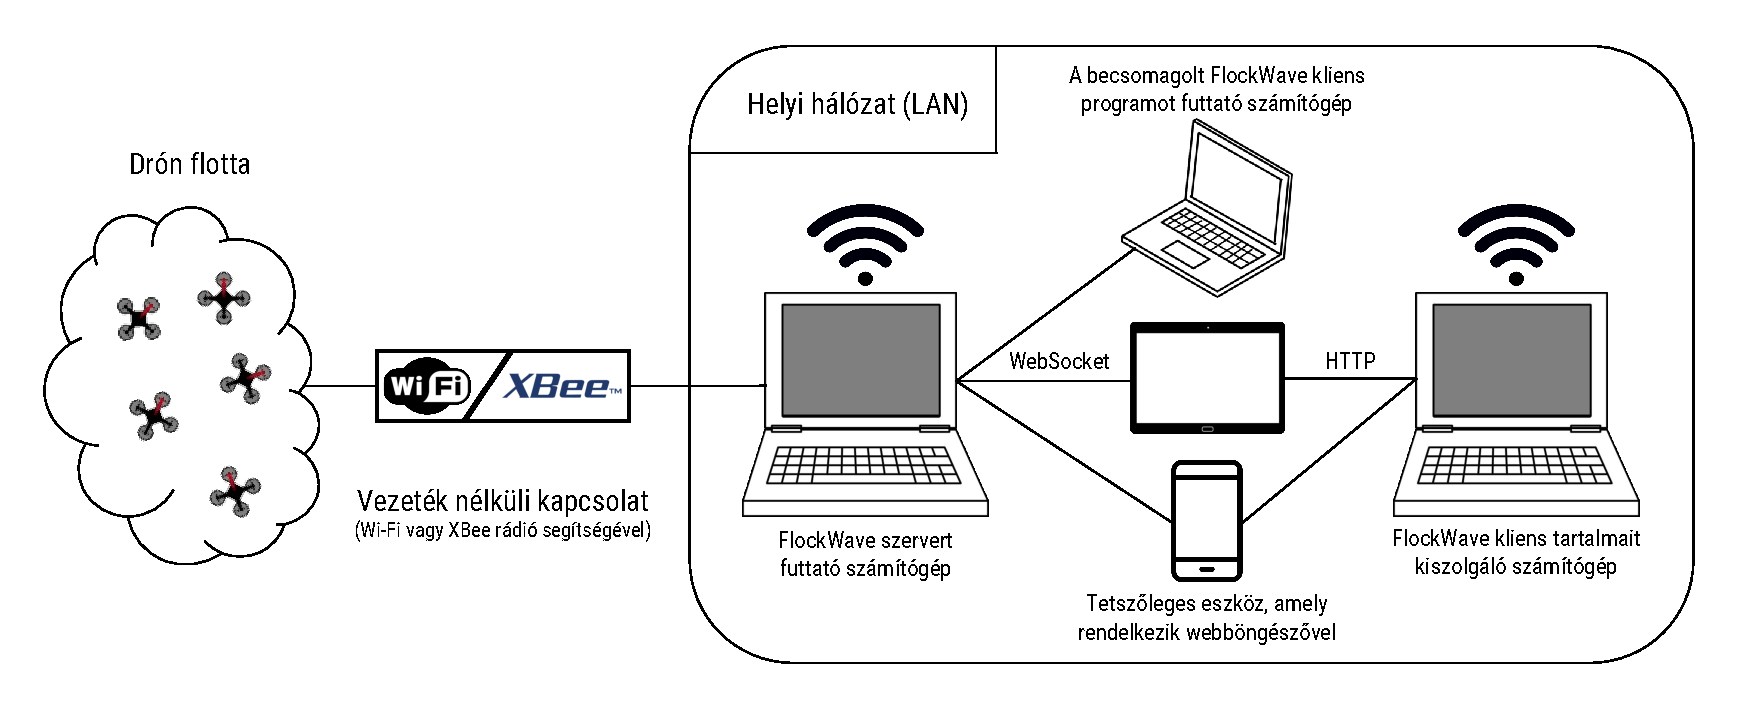
\includegraphics[width=\textwidth]{operational_structure_2.pdf}
  \caption{A rendszer felépítése}
\end{figure}

\textit{
  Megjegyzés: Természetesen semmi sem zárja ki, hogy a FlockWave szerver
  futtatását és a kliens tartalmának kiszolgálását, valamint akár egyben
  megjelenítését is ugyanaz a számítógép végezze.
}
